\chapter{Metodologia}

Para a realização do projeto, é necessário antes explicar as tecnologias usadas, e o por quê foram usadas. A primeira seção irá explicar como os dados estão disponíveis e de que informações eles carregam.  A segunda fala sobre a linguagem de programação utilizada para conseguir os dados, verificar se os dados estão completos, e armazena-los em um banco de dados. A terceira clarifica o que é um banco de dados, e porque foi utilizado.

\section{API do \textit{league of legends}}
A \textit{Riot Games}, desenvolvedora e dono do jogo \textit{League of Legends}, fornece uma Interface de Programação de Aplicativos ( do inglês \textit{Application Programming Interface} ) ou chamado de API para que terceiros consigam acessar dados sobre os jogos.

Para conseguir ter acesso à essa API, é necessário se cadastrar, entrar no \textit{site} na parte de desenvolvedores, disponível em http://developer.riotgames.com ( não sei se pode por link assim ).  Depois de cadastrado e de se credenciar no \textit{site}, deve ser clicado no botão para gerar uma chave API, que é válida por apenas alguns dias, a menos que cadastre o projeto, dessa maneira a chave é válida por um ano.

O acesso à essa API é por URL utilizando uma função disponível pela \textit{RIOT Games}. Neste trabalho, usaremos apenas a função \textit{MATCH-V3}, que é uma função que retorna os dados de uma partida já terminada.
Nas próximas subseções serão abordados o formato no qual a API disponibiliza os dados, e quais informações ela retorna com o uso do \textit{MATCH-V3} e quais serão usados no projeto.
\subsection{JSON}
(preciso achar outros autores para respaldarem)

A API do \textit{League of Legends} disponibiliza as informações no formato de Notação de Objeto JavaScript ( do inglês \textit{ JavaScript Object Notation.} ) ou JSON.
O JSON é um formato de dados que é escrito em forma de texto. O padrão JSON é um jeito de escrever as informações casando o nome das variáveis com um valor, ou em uma lista ordenada de valores. E o objeto em JSON é uma lista desordenada de valores \citep{json2}.
 
 
Segundo o \citeauthor{json2} "JSON [...] é uma formatação leve de troca de dados. Para seres humanos, é fácil de ler e escrever. Para máquinas, é fácil de interpretar e gerar." e continua explicando "JSON é em formato texto e completamente independente de linguagem, pois usa convenções que são familiares às linguagens C e familiares [...]. Estas propriedades fazem com que JSON seja um formato ideal de troca de dados."

\begin{figure}[!ht]
	\caption{Representação visual de um objeto em JSON}
	\begin{center}
		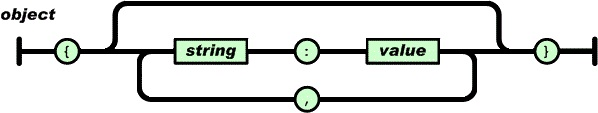
\includegraphics[width=15cm]{imagens/json.jpg}
	\end{center}
	\small{Fonte: \cite{json2}.}
	\label{fig:Json}
\end{figure}
 

\subsection{MATCH-V3}

A função \textit{MATCH-V3} é disponibilizada publicamente pela \textit{RIOT Games} e que retorna um conjunto de informações no formato JSON sobre a partida passada por parâmetro, quando essa partida existe no banco de dados da \textit{RIOT Games}. A Figura \ref{fig:match-v3} resume um exemplo de acesso utilizando a função acessando a URL  
\(https://br1.api.riotgames.com/lol/match/v3/matches/1381102031?api\_key=minhachave\) acessada em 21 de março de 2018, sendo que \(minhachave\) tem que ser substituída por uma chave privada válida.
\begin{figure}[!ht]
	\caption{Exemplo de retorno do uso da função \textit{MATCH-V3}}
	\begin{center}
		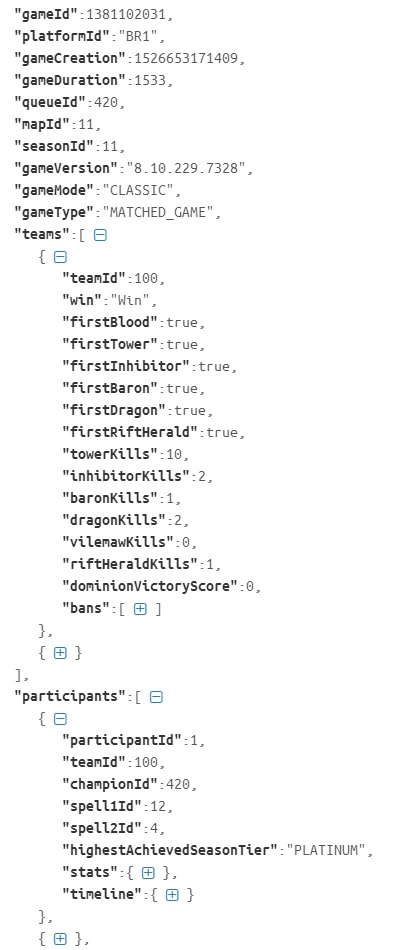
\includegraphics[width=9cm]{imagens/match-v3.jpg}
	\end{center}
	\small{Fonte: Autor.}
	\label{fig:match-v3}
\end{figure}

De todas essas informações retornadas pela função, as informações armazenadas para o projeto por participante são:
\begin{itemize}
\item \textit{gameId}. Identificador único da partida;
\item \textit{kills}, \textit{deaths} e \textit{assists}. Informações que falam, respectivamente, quantas vezes esse jogador matou, morreu e participou na morte de outrem;
\item \textit{win}. Se ele ganhou;
\item \textit{championId}. Qual campeão ele escolheu;
\item \textit{lane}. Em qual posição ele tava jogando;
\item \textit{platformId}. Em qual servidor ele jogava;
\item \textit{queueId}. E qual o tipo de partida.
\end{itemize}

Sabendo qual informação vamos armazenar, ficou escolhido a linguagem \textit{Python} para ser desenvolvido o algoritmo no qual obterá as informações de forma não manual e o sistema de gerenciamento de banco de dados MySQL. Na próxima seção será apresentado sobre banco de dados e na seção \ref{section:python} será esclarecido o que é linguagem de programação \textit{Python} e como foi usado. 


\section{Banco de Dados}
(continua)
\section{\textit{Python}}
\label{section:python}
\textit{Python} é uma linguagem de programação dentre muitas, assim como existem várias linguagens faladas e escritas por nós humanos, no mundo da computação, existem várias linguagens de programação, onde geralmente cada uma se destaca em pelo menos um quesito. 

(pegar algum autor para respaldar, e pegar algum texto dele falando sobre vantagens do \textit{Python}, que é interpretado e continua.)

Entendendo isso, foi criado um algoritmo para a aquisição dos dados de partidas pela API do \textit{League of Legends}, que usava a biblioteca \textit{requests} do \textit{Python} para conseguir acessar a API por URL's, e a biblioteca json também do \textit{Python} para transformar o Json retornado pela requisição da URL em um objeto em \textit{Python}.

O aplicativo verifica se a partida requisitada existe e se os dados necessários estão completo, salvando no banco de dados apenas as partidas válidas. O pseudo-codigo se encontra no Algoritmo \ref{alg:main-aqui}.

\
 %Código


\begin{algorithm}[H]
   \SetAlgoLined
     \Inicio{

		i = 1000000000; /* Esta é a \textit{id} de uma partida aleatória na ultima versão do jogo*/
            
		chave = minha chave privada de acesso;
            
        \uSe{Existe arquivo com ultimo partida lido}{
          	i = ultima partida lida;
        }
        \Repita{Até ser pausado}{    
            pedido = requisita URL Da API(i, chave);
            
            \uSe{pedido.status == 200}{ /* se a partida existe */
            	JSON = carrega JSON Do Pedido(pedido);
                
                \uSe{JSON é válido}{
                	Armazena os dados em um banco de dados;
                }
                
                i = i + 1;
                
                Salva i no arquivo;
            }
		}
    }
   \label{alg:main-aqui}
   \caption{\textsc{Aquisição dos dados das partidas}}
 \end{algorithm}

\

Onde com esse algoritmo foram armazenadas \numpartidas\ jogos válidos diferentes, e foi decidido usar apenas as partidas ranqueadas 5 contra 5, já que estas são as partidas responsáveis pela classificação dos jogadores dentro dos jogo, e as partidas não ranqueadas são consideradas como amistosas.
Com esse escopo, o número de partidas usados foram ao todo \partidasrankeds\ partidas ranqueadas diferentes, na tabela \ref{tab:subset-lol} é possível ver uma pequena fatia dos dados salvos.


\begin{table}[H]
\centering
\caption{Exemplo de \textit{subset} salvo no banco de dados}
\label{tab:subset-lol}
\resizebox{\textwidth}{!}{%
\begin{tabular}{cccccccccc}
match\_id  & kills & deaths & assists & win & champ\_id & lane   & player\_id & platform & type \\
1282000002 & 11    & 10     & 7       & 0   & 67        & BOTTOM & 16112724   & BR1      & 420  \\
1282000002 & 2     & 8      & 15      & 0   & 412       & BOTTOM & 18604874   & BR1      & 420  \\
1282000002 & 7     & 4      & 7       & 0   & 34        & MIDDLE & 19281809   & BR1      & 420  \\
1282000002 & 7     & 6      & 4       & 0   & 5         & JUNGLE & 21304223   & BR1      & 420  \\
1282000002 & 5     & 7      & 12      & 0   & 98        & TOP    & 651014     & BR1      & 420  \\
1282000002 & 0     & 6      & 23      & 1   & 44        & BOTTOM & 18592234   & BR1      & 420  \\
1282000002 & 19    & 5      & 5       & 1   & 222       & BOTTOM & 7170345    & BR1      & 420 
\end{tabular}%
}
\small{Fonte: Autor.}
\end{table}

Com esse número de partidas, foi feito um outro \textit{software}, para processamento dos dados, onde é contabilizado quantas vezes cada campeão jogou com outro campeão, seja no mesmo time ou no time adversário, calculado quantas vitória contra, e com o outro herói. Na tabela \ref{tab:matriz-subset} é possível ver um exemplo de como a estrutura fica apos o processamento dos dados, sendo \textit{id}, o identificador de cada campeão, e vj, vc, nj e nc sendo respectivamente as vitórias juntos, vitórias contra, número de jogos juntos, números de jogos contra.

\begin{table}[H]
\centering
\caption{Exemplo da matriz gerada apos o processamento dos dados}
\label{tab:subset-lol}
\label{tab:matriz-subset}
\resizebox{\textwidth}{!}{%
\begin{tabular}{@{}|c|c|c|c|c|c|c|c|c|c|c|c|c|c|@{}}
\toprule
\multicolumn{2}{|c|}{\multirow{2}{*}{id x id}} & \multicolumn{4}{c|}{1}                 & \multicolumn{4}{c|}{2}                                                              & \multicolumn{4}{c|}{3}                                                                \\ \cmidrule(l){3-14} 
\multicolumn{2}{|c|}{}                         & vj       & vc      & nj      & nc      & vj                 & vc                 & nj                  & nc                  & vj                  & vc                  & nj                  & nc                  \\ \midrule
\multirow{4}{*}{1}             & vj            & \multicolumn{4}{c|}{\multirow{4}{*}{}} & \multirow{4}{*}{7} & \multirow{4}{*}{3} & \multirow{4}{*}{13} & \multirow{4}{*}{11} & \multirow{4}{*}{11} & \multirow{4}{*}{23} & \multirow{4}{*}{17} & \multirow{4}{*}{33} \\ \cmidrule(lr){2-2}
                               & vc            & \multicolumn{4}{c|}{}                  &                    &                    &                     &                     &                     &                     &                     &                     \\ \cmidrule(lr){2-2}
                               & nj            & \multicolumn{4}{c|}{}                  &                    &                    &                     &                     &                     &                     &                     &                     \\ \cmidrule(lr){2-2}
                               & nc            & \multicolumn{4}{c|}{}                  &                    &                    &                     &                     &                     &                     &                     &                     \\ \midrule
\multirow{4}{*}{2}             & vj            & \multicolumn{4}{c|}{7}                 & \multicolumn{4}{c|}{\multirow{4}{*}{}}                                              & \multirow{4}{*}{5}  & \multirow{4}{*}{8}  & \multirow{4}{*}{9}  & \multirow{4}{*}{11} \\ \cmidrule(lr){2-6}
                               & vc            & \multicolumn{4}{c|}{8}                 & \multicolumn{4}{c|}{}                                                               &                     &                     &                     &                     \\ \cmidrule(lr){2-6}
                               & nj            & \multicolumn{4}{c|}{13}                & \multicolumn{4}{c|}{}                                                               &                     &                     &                     &                     \\ \cmidrule(lr){2-6}
                               & nc            & \multicolumn{4}{c|}{11}                & \multicolumn{4}{c|}{}                                                               &                     &                     &                     &                     \\ \midrule
\multirow{4}{*}{3}             & vj            & \multicolumn{4}{c|}{11}                & \multicolumn{4}{c|}{5}                                                              & \multicolumn{4}{c|}{\multirow{4}{*}{}}                                                \\ \cmidrule(lr){2-10}
                               & vc            & \multicolumn{4}{c|}{10}                & \multicolumn{4}{c|}{3}                                                              & \multicolumn{4}{c|}{}                                                                 \\ \cmidrule(lr){2-10}
                               & nj            & \multicolumn{4}{c|}{17}                & \multicolumn{4}{c|}{9}                                                              & \multicolumn{4}{c|}{}                                                                 \\ \cmidrule(lr){2-10}
                               & nc            & \multicolumn{4}{c|}{33}                & \multicolumn{4}{c|}{11}                                                             & \multicolumn{4}{c|}{}                                                                 \\ \bottomrule
\end{tabular}%
}
\small{Fonte: Autor.}
\end{table}

E com as informações já processados, foi montado um \textit{webapp}, que sera explicado na proxima secão, para uma melhor visualização dos dados obtidos.

\section{\textit{webapp}}

(continua...)

Com essa aplicação, é possível visualizar o resultado de todos os dados no banco de dados ou diminuir o escopo, filtrando alguns dados. Na figura \ref{fig:webapp} é possível ver um exemplo

\begin{figure}[h]
	\caption{Exemplo do uso do \textit{WEBAPP}}
	\begin{center}
		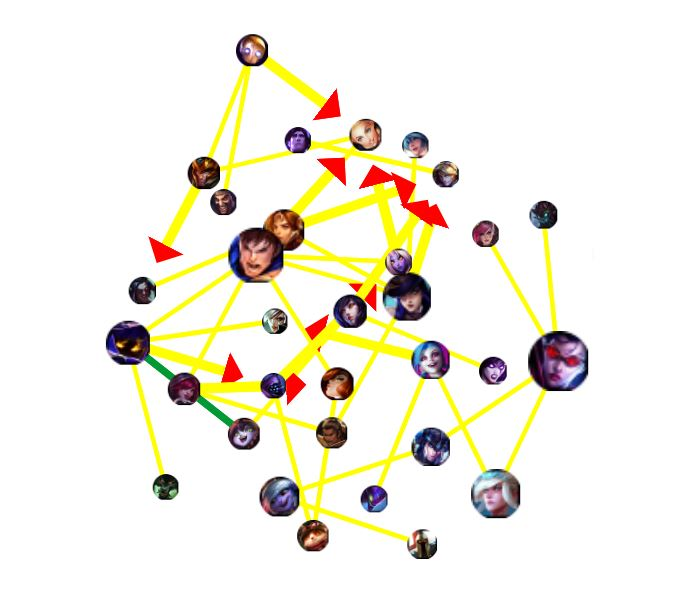
\includegraphics[width=12cm]{imagens/webservice.jpg}
	\end{center}
	\small{Fonte: Autor.}
	\label{fig:webapp}
\end{figure}
